\begin{table}[H]	
	\centering
	\def\arraystretch{1.25}
	\begin{tabular}{|m{5cm}|m{5cm}|m{5cm}|}
		\hline
		\textbf{Date} & \textbf{Tommaso Bianchi} &  \textbf{Federico Betti}\\ \hline
		28/11/17 &	3 &	3 \\ \hline
		29/11/17 &	1 &	1 \\ \hline
		30/11/17 &	4 &	4 \\ \hline
		01/12/17 &	2 &	2 \\ \hline
		02/12/17 &	2 & 0	 \\ \hline
		03/12/17 &	4 &  0\\ \hline
		04/12/17 &	1,5 & 0 \\ \hline
		05/12/17 &	6 &	6 \\ \hline
		06/12/17 &	5,5 & 0	 \\ \hline
		07/12/17 &	0 &	6 \\ \hline
		08/12/17 &	6 &	3,5 \\ \hline
		10/12/17 &	4 &	2 \\ \hline
		11/12/17 &	2,5 &	2,5 \\ \hline
		12/12/17 &	5 &	2,5 \\ \hline
		13/12/17 &	0 &	3,5 \\ \hline
		14/12/17 &	3 & 0	 \\ \hline
		15/12/17 &	5,5 &	1,5 \\ \hline
		16/12/17 &	3,5 &	6 \\ \hline
		17/12/17 &	5,5 &	5 \\ \hline
		19/12/17 &	5,5 &	5,5 \\ \hline
		20/12/17 &	0 &	2 \\ \hline
		21/12/17 &	4 & 0	 \\ \hline
		22/12/17 &	3 &	1 \\ \hline
		27/12/17 &	2,5 &	4 \\ \hline
		28/12/17 &	0 &	2 \\ \hline
		29/12/17 &	0 &	2 \\ \hline
		02/01/18 &	2 &	4 \\ \hline
		03/01/18 &	4 &	2 \\ \hline
		04/01/18 &	4 &	8,5 \\ \hline
		05/01/18 &	4 & 0	 \\ \hline
		06/01/18 &	0 &	2 \\ \hline
		07/01/18 &	6 &	6 \\ \hline
	\end{tabular}
	\caption{Effort Spent}
\end{table}



%\begin{figure}[H]
%	\centering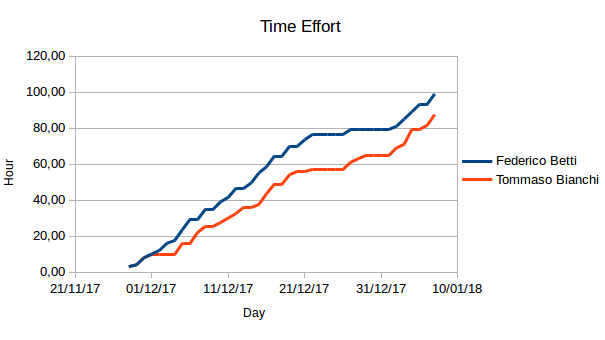
\includegraphics[width=\textwidth]{Images/TimeEffort.png}
%	\caption{Effort Spent}
%\end{figure}
